\documentclass[11pt,a4paper]{article}
\usepackage[left=2cm,right=2cm,top=2cm,bottom=2.3cm]{geometry}
\usepackage{amssymb,amsmath}
\usepackage[unicode,colorlinks]{hyperref}
\usepackage[pdftex]{graphicx}
\usepackage{wrapfig}

\usepackage[utf8]{input enc}
\usepackage[english, russian]{babel}

\numberwithin{equation}{section}

\newcommand{\nn}{\nonumber}
\newcommand{\pt}{\partial}
\newcommand{\grad}{\mathrm{grad}\,}
\newcommand{\rot}{\mathrm{rot}\,}
\renewcommand{\div}{\mathrm{div}\,}
\newcommand{\vn}{\vec{\nabla}}
\newcommand{\eps}{\epsilon}
\newcommand{\const}{\mathrm{const}}

\graphicspath{{./pics/}}
\title{Электродинамика}
\author{Игорь Шендерович\\\texttt{shender.i@gmail.com}}
\begin{document}
\maketitle

\section{Векторный анализ.}

Рассмотрим электрический заряд $q$, расположенный в какой-нибудь точке
в пространстве. Этот заряд создаёт статическое электрическое поле. По
закону Кулона его напряжённость выражается формулой
\begin{equation}
  \label{eq:coulomb}
  \vec{E}(\vec{r}) =k \frac{q \vec{r}}{r^3}.
\end{equation}

Видно, что вектор $\vec{E}$ существует в любой точке пространства, вне
зависимости от того, насколько далеко мы отошли от заряда. Это
позволяет ввести понятие \textit{векторного поля} --- вида материи,
который существует при наличии источника. В данном случае источником
электрического поля является заряд $q$. Позднее мы увидим, что
магнитное поле, несмотря на отсутсвие одиночных источников, также
допускает такую интерпретацию. С этого момента мы будем говорить не о
напряжённости $\vec{E}$, а об электрическом (или магнитном) поле
$\vec{E}(x,y,z,t)$ (или $\vec{B}(x,y,z,t)$). Заметим, что поле может
зависеть как от точки пространства, так и от времени. 

Поскольку вектор определяется своими проекциями, то задать векторное
поле --- то же самое, что задать три его проекции. Таким образом,
электрическое поле $\vec{E}$ --- три функции четырёх переменных. 

Понятно, что в природе существуют и другие поля, не обязательно
векторные. Рассмотрим, например, поле температур $T(x,y,z,t)$. Это
тоже поле (т.к. температуру можно определить в любой точке
пространства), но \textit{скалярное}, поскольку температура не имеет
направления, а определяется лишь числовым значением. 

Другой пример векторного поля, более приближенный к реальности ---
поле скоростей жидкости. Каждой <<частице>> движущейся жидкости можно
сопоставить векторную функцию $\vec{v}(\vec{r},t)$, которая описывает
скорость данной частички. По определению, это векторное поле
скоростей. Мы увидим в дальнейшем, что многие свойства этого поля
жидкости переносятся и на электродинамику. 

Электрические и магнитные (или просто электромагнитные) поля устроены
довольно сложно, но при этом связь между значениями полей в двух
соседних точках довольно проста. Задача наших упражнений --- вывести
эту связь в наиболее общем виде. 

\begin{wrapfigure}{r}{40mm}
  \vspace{-1cm}
  \begin{center}
  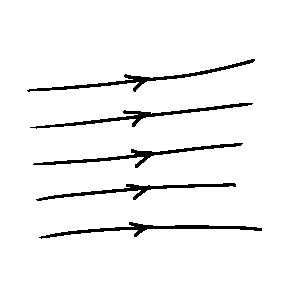
\includegraphics[width=4cm]{lines.pdf}  
  \end{center}
  \vspace{-1cm}
  \caption{Силовые линии.}
  \label{fig:force_lines}
  \vspace{-1.1cm}
\end{wrapfigure}

Как можно зрительно представлять поля? Лучше всего это делать с
помощью \textbf{силовых линий} --- таких линий, касательные к которым в
каждой точке будут давать направление вектора напряжённости в этой
точке. 

Чтобы изобразить на подобной картинке величину модуля вектора
напряжённости, можно условиться рисовать линии гуще в тех местах, где
абсолютная величина этого вектора больше. 

\subsection{Поток.}
\label{sec:flux}

Векторные поля обладают двумя очень важными характеристиками, которые
мы будем использовать при описании. Первая из них --- \textbf{поток}. 

Рассмотрим, к примеру, поток жидкости через некоторую ограниченную
поверхность. Можно задать себе вопрос --- сколько жидкости втекает
(вытекает) через эту поверхность площади $S$? 

Это количество можно посчитать следующим образом. Разобъём нашу
поверхность на много кусочков с площадью $dS$ каждый. К каждому
кусочку проведём вектор нормали $\vec{n}$ (так, чтобы он смотрел
наружу поверхности, а не внутрь). Тем самым, у каждого кусочка площади
будет задана ориентация. Для краткости совокупность данных о площади
кусочка и векторе нормали можно записывать в виде одного вектора
$d\vec{S}$ --- это вектор, по модулю равный $dS$, с направлением,
совпадающим с $\vec{n}$.

\begin{wrapfigure}{r}{40mm}
  \vspace{-1cm}
  \begin{center}
    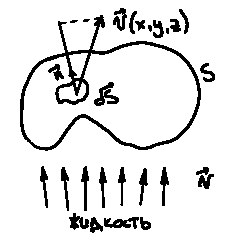
\includegraphics[width=4cm,height=4cm]{flux.pdf}
  \end{center}
  \vspace{-0.7cm}
  \caption{Поток.}
  \label{fig:flux}
\end{wrapfigure}

Спроецируем на направление этого вектора наше поле $\vec{v}$. Операция
проектирования проще всего выглядит как скалярное произведение
$\vec{v} \cdot d \vec{S}$. Действительно, по определению, скалярное
произведение равно $d\Phi = v \cdot dS \cdot \cos \alpha$, где $\alpha$ ---
угол между вектором $\vec{v}$ и нормалью $\vec{n}$. Теперь
просуммируем подобные выражения по всей поверхности, иными словами,
проинтегрируем по ней:

\begin{equation}
  \label{eq:def_flux}
  \Phi \equiv \int_S \vec{v} \cdot d \vec{S}.
\end{equation}

По определению, это скалярное произведение и называется потоком $\Phi$ 
векторного поля $\vec{v}$. Можно интерпретировать это определение и
таким способом: поток векторного поля равен среднему значению
нормальной компоненты поля $\vec{v}$, умноженному на величину площади
$S$. 

Если, например, поле устроено так, что не зависит от конкретной точки
(всюду постоянное поле), то формула для расчёта потока может быть
сильно упрощена. Пусть, скажем, поле всюду направлено по нормали к
поверхности (пример --- электрическое поле точечного заряда, а
поверхность --- сфера). Тогда в любой точке скалярное произведение
превращается в обычное (т.к. $\cos 0 = 1$), и функцию $v$ можно
вынести за знак интеграла. Интеграл же от $dS$ даст просто площадь
поверхности. Таким образом, в этом простейшем случае поток станет
равен $\Phi = vS$. 

В более сложных случаях (которые обычно и встречаются в природе),
вычисление потока по определению --- довольно сложная задача. К
счастью, у нас будет \textbf{теорема Гаусса}, которая позволяет свести
вычисление потока к относительно простым операциям. 

\subsection{Циркуляция.}
\label{sec:curl}

Опять представим себе поле скоростей, описывающее поток
жидкости. Зададимся таким вопросом: циркулирует ли эта жидкость? Иными
словами, существует ли её вращательное движение вдоль некоторого
замкнутого геометрического контура? 

\begin{wrapfigure}{r}{40mm}
  \vspace{-1.5cm}
  \begin{center}
    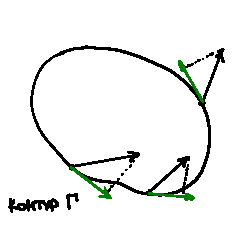
\includegraphics[width=4cm,height=4cm]{curl.pdf}
  \end{center}
  \vspace{-0.7cm}
  \caption{Циркуляция.}
  \label{fig:curl}
\end{wrapfigure}


По определению, \textbf{циркуляцией} $C$ называется скорость жидкости вдоль
контура, умноженная на длину этого контура. Как и в случае с потоком,
можно думать про эти величины как про средние; более аккуратное
определение можно получить, опять пользуясь понятием проекции. 

Рассмотрим участок контура длиной $dl$. С ним, как и с кусочком
площадки, можно связать направление. Рассмотрим вектор $d\vec{l}$ ---
это вектор, модуль которого равен $dl$, а направление совпадает с
направлением касательной в данной точке. Теперь спроецируем наше
векторное поле $\vec{v}$ на этот вектор $d\vec{l}$. Сделать это можно
так же, как и в случае с потоком, т.е. взять скалярное
произведение. Теперь просуммируем это по всему контуру:

\begin{equation}
  \label{eq:curl}
  C \equiv \oint_\Gamma \vec{v} \cdot d \vec{l}.
\end{equation}

Пользуясь понятиями потока и циркуляции, мы опишем все законы
электродинамики, т.е. получим уравнения Максвелла. 

\subsection{Произведение векторов.}
\label{sec:vector_product}

Разберём подробнее операции с векторами. Нам понадобится умение
перемножать вектора двумя способами, дифференцировать их и
интегрировать. 

Два вектора $\vec{a}$ и $\vec{b}$ можно перемножить двумя способами:
скалярно и векторно. \textbf{Скалярное произведение} определяется через
компоненты этих векторов:

\begin{equation}
  \label{eq:def_scalar_product}
  \vec{a} \cdot \vec{b} \equiv a_x b_x + a_y b_y + a_z b_z.
\end{equation}

С помощью скалярного произведения можно также определить модуль
вектора: это корень из скалярного произведения вектора на самого себя.

\begin{equation}
  \label{eq:def_modulus_vector}
  |a| \equiv \sqrt{\vec{a} \cdot \vec{a}}.
\end{equation}

Также можно образовать \textbf{векторное произведение}: такое
произведение двух векторов, результатом которого является снова
вектор. Модуль этого вектора равен

\begin{equation}
  \label{eq:def_cross_product}
  | \vec{a} \times \vec{b}| = |\vec{a}| |\vec{b}| \sin \alpha,  
\end{equation}
а направление задаётся правилом правой руки. Угол $\alpha$ --- угол
между векторами. 

\begin{wrapfigure}{r}{40mm}
  \vspace{-1.5cm}
  \begin{center}
    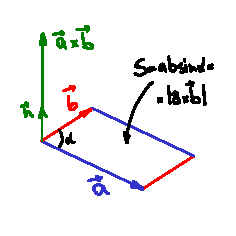
\includegraphics[width=4cm,height=4cm]{cross.pdf}
  \end{center}
  \vspace{-0.7cm}
  \caption{Векторное произведение.}
  \label{fig:curl}
  \vspace{-1cm}
\end{wrapfigure}

Свойства этого произведения довольно просты. Во-первых, если вектора
$\vec{a}$ и $\vec{b}$ коллинеарны, то $\vec{a} \times
\vec{b}=0$. Во-вторых, модуль этого вектора совпадает с площадью
параллелограмма, натянутого на вектора $\vec{a}$ и $\vec{b}$.

А можно ли записать определение векторного произведения в координатах,
подобно \eqref{eq:def_scalar_product}? Оказывается, можно. Именно, 

\begin{eqnarray}
  \label{eq:def_cross_product_components}
  \nn
  (\vec{a} \times \vec{b})_x &=& a_y b_z -a_z b_y,\\
  (\vec{a} \times \vec{b})_y &=& a_z b_x -a_x b_z,\\
  \nn
  (\vec{a} \times \vec{b})_z &=& a_x b_y -a_y b_x.
\end{eqnarray}

Запомнить это правило довольно просто: для i-ой компоненты нужно
устроить циклическую перестановку из индексов (xyz), где нужный индекс
стоит на i-ом месте. 

Понять, откуда взялось это правило, довольно просто. Рассмотрим три
орта $\vec{i},\vec{j},\vec{k}$. Применяя к ним правило
\eqref{eq:def_cross_product}, получим, что $\vec{i} \times \vec{j} =
\vec{k}$, \ldots. Расписывая вектор $\vec{a} = a_x \vec{i} + a_y
\vec{j} + a_z \vec{k}$, а вектор $\vec{b}$ аналогично, получим
требуемые свойства \eqref{eq:def_cross_product_components}. 

\subsection{Градиент. Оператор $\nabla$.}
\label{sec:gradient}

Предположим, что у нас имеется для начала скалярное поле, типа поля
температур. Мы хотим как-то описать изменение температуры $T(x,y,z,t)$
в пространстве. В отличие от похожей задачи --- изменения температуры
по времени --- нам нужно дифференцировать не по времени, а придумать
что-то другое, более подходящее к данному случаю.

Понятно, что если бы у нас была одна координата, то сработала бы
производная $dT/dx$, потому что именно она бы определяла скорость
изменения температуры вдоль оси $x$. В данном случае нам понадобятся
три производных 

\begin{equation}
  \label{eq:def_grad_1}
  \frac{\pt T}{\pt x}, \quad   \frac{\pt T}{\pt y}, \quad   \frac{\pt
    T}{\pt z},
\end{equation}
из которых можно сделать вектор. Вектор можно соорудить естественным
способом. Вспомним, что у нас есть три орта
$\vec{i},\vec{j},\vec{k}$. Построим вектор \textbf{градиента} по такому
правилу:

\begin{equation}
  \label{eq:def_grad_2}
  \grad T (x,y,z) \equiv \nabla T \equiv \frac{\pt T}{\pt x} \vec{i} +  \frac{\pt T}{\pt y}
  \vec{j} +  \frac{\pt T}{\pt z} \vec{k}.
\end{equation}

Таким образом, можно сказать, что градиент скалярного поля --- это
аналог производной, только в числе измерений больше одного. 

Заметим, что градиент, будучи вектором, явно зависит от
направления. Это сооветствует тому факту, что температура в разных
направлениях пространства может вестии себя по-разному. Таким образом,
градиент температуры $\grad T$ --- векторное поле, образованное из скалярного
поля самой температуры $T$.

Физический смысл градиента такой: в каждой точке пространства он
указывает направление, в котором температура меняется быстрее всего. 

Оказывается, что у градиента есть ещё одна интерпретация. Она ведёт к
обобщению известной теоремы \textbf{Ньютона--Лейбница}. Эта теорема
устроена примерно так. Представим себе, что у нас есть материальная
точка, двигающаяся в пространстве. Её координаты мы будем
характеризовать радиус--вектором $\vec{r}(t)$. Вычислим скорость этой
материальной точки; по определению, она равна $\vec{v} (t) = d
\vec{r}(t) / dt$. Что получится, если мы теперь проинтегрируем эту
скорость по времени от момента $t_1$ до $t_2$? 

\begin{equation}
  \label{eq:newton_leibnitz}
  \int_{t_1}^{t_2} \vec{v}(t) \, dt = \int_{t_1}^{t_2}
  \frac{d\vec{r}(t)} {dt} \, dt = \int_{t_1}^{t_2} d\vec{r}(t) =
  \vec{r}(t_2) - \vec{r}(t_1) = \Delta \vec{r}.
\end{equation}

То есть, если проинтегрировать скорость, получится перемещение. Более
общо: если проинтегрировать производную некоторой функции $f(t)$,
получится изменение этой самой функции $f(t)$. 

Эта теорема естественным образом ограничена на прямую линию (интеграл
вдоль прямой). Что будет, если мы захотим проинтегрировать что-нибудь
(а точнее, какой--нибудь вектор) вдоль произвольной кривой? 

\begin{wrapfigure}{r}{40mm}
  \vspace{-1.2cm}
  \begin{center}
    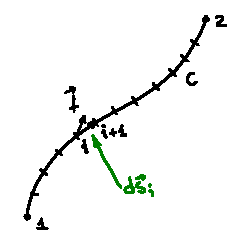
\includegraphics[width=4cm,height=4cm]{curve_int.pdf}
  \end{center}
  \vspace{-0.7cm}
  \caption{Интеграл вдоль кривой.}
  \label{fig:curve_int}
\end{wrapfigure}


В этом случае нам нужно описать процедуру интегрирования вдоль
кривой. Рассмотрим кусочек дуги кривой $\Delta l_i$. Пускай значение функции
на нашем кусочке равно $f_i$. Тогда интегралом вдоль кривой $C$
называется такое выражение:

\begin{equation}
  \label{eq:def_curve_int_1}
  \int_C  \vec{f} \cdot d\vec{l} \equiv \lim_{N\to \infty} \sum_{i=0}^N f_i \Delta l_i. 
\end{equation}

В общем, это что-то, аналогичное стандартному определению интеграла,
только нужно учитывать, что $f_i$ --- значение функции на этом
отрезке. В нашем случае вместо скаляра $f_i$ уместно взять скалярное
произведение 

\begin{equation}
  \label{eq:def_curve_int_2}
  \grad \phi \cdot d\vec{l}_i.
\end{equation}

Мы уже знаем, что градиент показывает, насколько быстро меняется
функция в данном направлении. Таким образом, если мы спроецируем
градиент на какое-то выделенное направление, мы получим скорость
изменения функции в этом направлении. Проецирование делатся в точности
скалярным произведением \eqref{eq:def_curve_int_2}. Таким образом,
уравнение \eqref{eq:def_curve_int_2} даёт изменение скалярного поля в
направлении $d\vec{l}_i$: $\phi(i+1) - \phi(i)$, где $\phi(i)$ ---
значение поля в точке $i$. Суммируя все такие изменения, получаем, что
сумма \eqref{eq:def_curve_int_1} превращается в конечное изменение 

\begin{equation}
  \label{eq:def_curve_int_3}
  \int_C \grad \phi \cdot d\vec{l} = \phi(2) - \phi(1).
\end{equation}

Таким образом, мы видим, что у градиента есть такой смысл: будучи
проинтегрирован по какой-либо кривой, он даёт изменение конечное
изменение скалярной функции вдоль этой кривой. 

Заметим попутно, что интеграл от градиента, очевидно, не зависит от
кривой, вдоль которой мы интегрируем. Действительно, правая часть
уравнения \eqref{eq:def_curve_int_3} зависит только от значений поля
$\phi$ в точках 1 и 2, и больше не от чего. Очевидно, что значения
поля в этих точках не зависят от того, по какому пути мы в эти точки
пришли. 

Что будет, если мы придём из точки 1 в точку 2 по красному пути, а
уйдём обратно по синему? Мы опишем замкнутый контур. 

\begin{wrapfigure}{r}{40mm}
  \vspace{-1.5cm}
  \begin{center}
    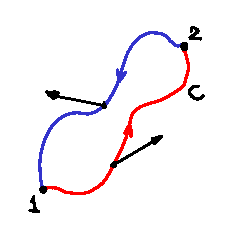
\includegraphics[width=4cm,height=4cm]{path_indep.pdf}
  \end{center}
  \vspace{-0.7cm}
  \caption{Замкнутый контур.}
  \label{fig:path_indep}
\end{wrapfigure}

Пройдём по красному контуру от точки 1 до точки 2. При этом значение
интеграла \eqref{eq:def_curve_int_3} даст нам, как и положено, $\phi(2)
- \phi(1)$. Теперь пройдём от точки 2 до точки 1 по синему
контуру. Интеграл даст на этот раз $\phi(1) - \phi(2)$. В итоге наших
прогулок по разноцветным контурам мы придём обратно в точку 1, при
этом значение интеграла по замкнутому контуру будет равно 0. Опять же,
заметим, что он конкретной формы этого контура ничего не зависит. 

Таким образом, мы доказали, что интеграл от градиента по замкнутому
контуру равен нулю, и от контура не зависит. Или, вспоминая
определение циркуляции \eqref{eq:curl}, мы доказали, что циркуляция
градиента равна нулю.

\begin{equation}
  \label{eq:int_grad}
  \oint \grad \phi \cdot  d\vec{l} =0.
\end{equation}

В дальнейшем этот факт нам поможет. 

Напоследок продемонстрируем один трюк, ради которого (отчасти) это всё
и затевалось. Обозначим \emph{формально} буквой $\nabla$ такую
операцию:

\begin{equation}
  \label{eq:def_nabla}
  \vec{\nabla} \equiv \frac{\pt}{\pt x} \vec{i} +  \frac{\pt}{\pt y}
  \vec{j} +  \frac{\pt}{\pt z} \vec{k}.
\end{equation}

Буква $\vec{\nabla}$ теперь играет роль \textbf{оператора градиента},
т.е. не самостоятельной буквы, а чего-то, что имеет смысл только в
паре с функцией, к которой она применяется. Оператор градиента
<<ждёт>> функцию, которую ему надо продифференцировать. Из формулы
\eqref{eq:def_grad_2} видно, что градиент можно получить, действуя
оператором градиента на наше скалярное поле.

Очевидно, что, будучи вектором, оператор $\vec{\nabla}$ может быть применён
не только к скалярам (типа поля температуры), но и к векторам,
порождая объекты с очень прозрачным физическим смыслом. 

\subsection{Дивергенция.}
\label{sec:divergence}

Первое, что мы можем сделать с вектором $\vec{\nabla}$ и каким-то
векторным полем $\vec{A}$ --- скалярно их перемножить. Как следует из
определения, должен получиться скаляр. Посмотрим, так ли это.

\begin{equation}
  \label{eq:def_divergence}
  \div \vec{A} \equiv \vec{\nabla} \cdot \vec{A} = \frac{\pt}{\pt x}
  A_x +  \frac{\pt}{\pt y} A_y +  \frac{\pt}{\pt z} A_z = \frac{\pt
    A_x}{\pt x} +  \frac{\pt A_y}{\pt y} +  \frac{\pt A_z}{\pt z}.
\end{equation}

Скалярная величина, которую мы получили, называется
\textbf{дивергенцией}. Фактически, оператор $\vec{\nabla}$, скалярно
умноженный на $\vec{A}$, дифференцирует каждую из компонент вектора
$\vec{A}$ по соответствующей координате и складывает результаты без
учёта направления. Этим он и отличается от градиента: градиент,
напомним, даёт вектор. 

Итак, если градиент скалярному полю сопоставляет векторное, то
дивергенция векторному полю сопоставляет скалярное. 

Нет ли случайно у дивергенции какого-нибудь внятного физического
смысла? Разумеется, есть, иначе зачем бы она нам понадобилась!

Чтобы понять этот физический смысл, нам понадобится вспомнить понятие
потока \eqref{eq:def_flux}. Рассмотрим какое--нибудь тело, через
которое проходит векторное поле. Разобъём тело на маленькие одинаковые
кубики. Рассмотрим маленький кубик со сторонами $\Delta x$, $\Delta
y$, $\Delta z$. Пускай в пространстве есть какое-то векторное поле
$\vec{A}$. Вычислим его поток (наружу) через поверхность этого кубика.

У поверхности кубика 6 граней. Можно вычислить поток через каждую из
них. Поскольку грани --- маленькие квадраты, вычисление будет
несложным. Например, поток через грань 1 равен

\begin{equation}
  \label{eq:theorem_divergence_1}
  \Phi_1 = -\int A_y (x,y,z) dx dz.
\end{equation}
(знак минус появился от того, что в грань 1 наше поле \emph{входит},
так что поток \emph{наружу} будет со знаком минус). Это выражение
можно упростить: так как мы считаем наш кубик маленьким, то можно
считать, что на грани функция $A_y$ примерно постоянная; раз так, то
её можно вытащить за знак интеграла. Останется лишь интеграл по
площади грани, который равен собственно площади $\Delta x \Delta z$. 

\begin{wrapfigure}{r}{40mm}
  \vspace{-1.2cm}
  \begin{center}
    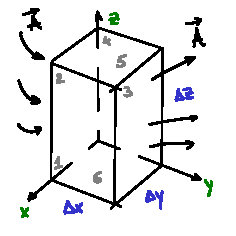
\includegraphics[width=4cm,height=4cm]{div.pdf}
  \end{center}
  \vspace{-0.7cm}
  \caption{Вычисление потока.}
  \label{fig:div}
  \vspace{2cm}
\end{wrapfigure}

Итого, получаем, что поток через грань 1 равен

\begin{equation}
  \Phi_1 = - A_y \Delta x \Delta z. 
\end{equation}

Рассмотрим теперь поток наружу через грань 3:

\begin{equation}
  \Phi_3 = \int A_y (x,y + \Delta y,z) dx dz = A_y (x,y+\Delta y,z)
  \Delta x \Delta z.
\end{equation}

Сложим теперь потоки $\Phi_1 + \Phi_3$ --- это логично сделать, потому
что у них есть много общего. 

\begin{equation}
  \label{eq:theorem_divergence_2}
  \Phi_1 + \Phi_3 = \Delta x \Delta z \left(A_y(y+\Delta y) - A_y
    (y)\right) \approx \Delta x \Delta z \Delta y \frac{\pt A_y}{\pt y}.
\end{equation}

Здесь мы заменили разность полей на двух гранях производной потому,
что кубик считается маленьким и такая замена не внесёт существенной
ошибки. Аналогичные операции можно провернуть и для остальных четырёх
граней; ответ для полного потока $\Phi$ совсем не удивителен:

\begin{equation}
  \label{eq:theorem_divergence_3}
  \Phi = \Delta x \Delta y \Delta z
  \left(
    \frac{\pt A_x}{\pt x} + 
    \frac{\pt A_y}{\pt y} + 
    \frac{\pt A_z}{\pt z}
  \right) = \Delta V \div \vec{A}. 
\end{equation}

Таким образом, физический смысл дивергенции такой: это поток
векторного поля, отнесённый к единице объёма $\Delta V$. Можно
сказать, что дивергенция меряет <<удельную величину>> потока, измеряя,
насколько мощный источник поля мы имеем. 

Более того, если мы теперь проинтегрируем равенство
\eqref{eq:theorem_divergence_3} по всему объёму тела и вспомним
определение потока \eqref{eq:def_flux}, мы получим ещё
одно соотношение, известное как \textbf{теорема Гаусса--Остроградского}:

\begin{equation}
  \label{eq:theorem_gauss_ostograd}
  \int_V \div \vec{A}\, dV =  \int_S \vec{A} \cdot  d\vec{S}.
\end{equation}

Заметим, что это соотношение чем-то похоже на теорему о градиенте
\eqref{eq:def_curve_int_3}: в правой части стоит что-то, размерности
на единицу меньшей, чем в левой части. Теперь если вы хотите сосчитать
поток какого--нибудь поля, у вас есть два варианта: либо вы честно его
считаете и берёте поверхностный интеграл, либо вы считаете дивергенцию
и берёте интеграл по объёму. Точно то же самое было в случае
градиента: либо считать интеграл вдоль кривой, либо считать приращение
функции вдоль этой же кривой.

Вскоре мы выясним, что есть ещё одна теорема похожего типа. Но для
начала посмотрим, на что ещё может сгодиться оператор $\vn$. 

\subsection{Ротор.}
\label{sec:curl}

Что ещё можно смастерить из оператора $\vec{\nabla}$ и вектора?
Помимо скалярного произведения, которое приводит к дивергенции, можно
сделать векторное произведение; в итоге получится вектор. Какие же у
него будут компоненты? Из формул \eqref{eq:def_cross_product} и
\eqref{eq:def_nabla} получаем: 

\begin{eqnarray}
  \label{eq:def_curl}
  \nn
  (\vec{\nabla} \times \vec{A})_x &=& \frac{\pt A_z}{\pt y} -  \frac{\pt
    A_y}{\pt z},\\
  (\vec{\nabla} \times \vec{A})_y &=& \frac{\pt A_x}{\pt z} -  \frac{\pt
    A_z}{\pt x},\\
  \nn
  (\vec{\nabla} \times \vec{A})_z &=& \frac{\pt A_y}{\pt x} -  \frac{\pt
    A_x}{\pt y}.
\end{eqnarray}

Вектор $\rot \vec{A} \equiv \vn \times \vec{A}$ называют
\textbf{ротором} или \textbf{вихрем}. Название выбрано неслучайно:
физический смысл этого вектора тесно связан с вихрями в потоке
жидкости (или в любом другом векторном поле).

Можно ли как-то выяснить физический смысл ротора аналогично
дивергенции и градиенту? Сейчас мы получим нечто, аналогичное теореме
Гаусса--Остроградского. Если в случае с дивергенцией мы интегрировали
поле по поверхности маленького кубика, то в случае с ротором надо
интегрировать по границе маленького квадрата (так подсказывает наша
интуиция).

\begin{wrapfigure}{r}{40mm}
  \vspace{-0.8cm}
  \begin{center}
    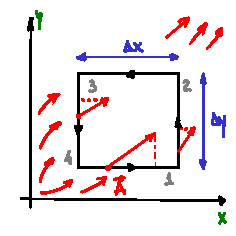
\includegraphics[width=4cm,height=4cm]{stokes.pdf}
  \end{center}
  \vspace{-0.7cm}
  \caption{Вычисление циркуляции.}
  \label{fig:stokes}
  \vspace{2cm}
\end{wrapfigure}


Рассмотрим, например, квадрат, расположенный в плоскость $xy$ со
сторонами $\Delta x$, $\Delta y$. Вычислим циркуляцию поля $\vec{A}$
по этому квадрату. Также как и в случае с потоком, полная циркуляция
складывается из циркуляций по каждому ребру. Посмотрим, например, на
ребро 1. Циркуляция по нему равна

\begin{equation}
  \label{eq:theorem_curl_1}
  C_1 = \int A_x (x,y) d x = A_x (x,y) \Delta x. 
\end{equation}

Здесь мы, как и в предыдущем пункте, воспользовались тем, что
квадратик маленький, а значит, поле на его ребре можно считать
постоянным вдоль ребра. Коль так, то поле можно вынести за знак
интеграла, ну а интеграл от $dx$ даст просто длину ребра. Проводя
аналогичную операцию для остальных рёбер, получим в сумме для
циркуляции

\begin{equation}
  \label{eq:theorem_curl_2}
  C_{xy} = C_1 + \ldots C_4 = \Delta x
  \left(
    A_x (x,y) - A_x(x,y+\Delta y)
  \right) + \Delta y
  \left(
    A_y (x+\Delta x, y) - A_y (x,y)
  \right).
\end{equation}

Раскладывая разность в скобках (наш контур считается малым), получим:

\begin{equation}
  \label{eq:theorem_curl_3}
  C_{xy} = \Delta x \Delta y \left(\frac{\pt A_y}{\pt x} - \frac{\pt A_x}{\pt y}\right).
\end{equation}

У нас получилось, что циркуляция поля вдоль контура, лежащего в
плоскости $xy$ равна площади этого контура $\Delta x \Delta y$,
умноженной на компоненту $z$ ротора поля $C$ (см. формулу
\eqref{eq:def_curl}). Компонента $z$ в данном случае --- нормальная
составляющая ротора по отношению к плоскости $xy$. Таким образом,
можно написать, что
\begin{equation}
  \label{eq:theorem_curl_4}
  \oint \vec{A} \cdot d\vec{l} = \rot \vec{A} \cdot \vec{n}\, \Delta S.
\end{equation}

Если теперь просуммировать циркуляции по всем маленьким контурам на
нашей поверхности $S$, получится \textbf{теорема Стокса}:

\begin{equation}
  \label{eq:theorem_curl_5_stokes}
  \oint \vec{A} \cdot d \vec{l} = \int_S \rot \vec{A} \cdot \vec{n} \,
  dS = \int_S \rot \vec{A} \cdot d\vec{S}.
\end{equation}

Опять, по аналогии с дивергенцией, заметим, что теорема связывает
нечто одномерное по сути (циркуляцию) с чем-то двумерным (интеграл по
поверхности от ротора). В каком-то смысле, теорема о градиенте
\eqref{eq:def_curve_int_3}, теорема Гаусса--Остроградского
\eqref{eq:theorem_gauss_ostograd} и теорема Стокса
\eqref{eq:theorem_curl_5_stokes} --- частные случаи одного более
общего соотношения, про которое здесь мы говорить не будем. 

\subsection{Манипуляции с $\vn$.}
\label{sec:nabla}

Сейчас мы начнём получать дивиденды от записи векторных операций через
оператор $\vn$. Попробуем составить всякие комбинации с двумя
операторами $\vn$. Например, возьмём скалярное поле $\phi$, возьмём
его градиент (получится векторное поле), от получившегося сосчитаем
ротор. Кратко это записывается так:

\begin{equation}
  \vn \times (\vn \phi).
\end{equation}

Мы можем немедленно вычислить это произведение. Дело в том, что скобки
можно расставлять как угодно (произведение ассоциативно), поэтому
получаем, что $\vn \times (\vn \phi) = (\vn \times \vn) \phi
=0$. Здесь мы воспользовались тем, что векторное произведение вектора
самого на себя равно нулю (т.к. <<угол>> между векторами равен
нулю). Итак, мы получили следующее равенство: 

\begin{equation}
  \label{eq:rot_grad}
  \vn \times (\vn \phi) = \rot \grad \phi = 0.
\end{equation}

Если мы применим к вектору $\grad \phi$ теорему Стокса
\eqref{eq:theorem_curl_5_stokes}, то получится

\begin{equation}
  \label{eq:stokes_gradient}
  \oint \grad \phi \cdot d\vec{l} = \int \rot \grad \phi \cdot
  d\vec{S} = 0.
\end{equation}

То есть, циркуляция градиента всегда равна нулю. Вспомним, что мы уже
видели это свойство в формуле \eqref{eq:int_grad}. Там мы её
доказывали напрямую, руками. А с помощью формальной операции $\vn$ и
теоремы Стокса мы получили это соотношение бесплатно.

Рассмотрим теперь комбинацию $ \vec{A} \cdot (\vec{A} \times
\vec{B})$. Вектор $\vec{A} \times \vec{B}$ перпендикулярен $\vec{A}$
(см. рис. \ref{fig:curl}), поэтому это произведение равно
нулю. Возьмём теперь в качестве $\vec{A} = \vn$, а в качестве
$\vec{B}$ какое--нибудь векторное поле $\vec{X}$. Получаем

\begin{equation}
  \label{eq:div_rot}
  \vn \cdot (\vn \times \vec{X}) = 0 = \div \rot \vec{X}.
\end{equation}

Применим к вектору $\rot \vec{X}$ теорему Гаусса--Остроградского
\eqref{eq:theorem_gauss_ostograd}:

\begin{equation}
  \label{eq:gauss_rot}
  \int_S \rot \vec{X} \cdot d\vec{S} = \int_V \div \rot \vec{X}\, dV = 0.
\end{equation}

Итак, мы получили, что поток вектора $\rot \vec{X}$ всегда равен
нулю. Это значит, что вихревое поле не создают никакие источники:
силовые линии не имеют начала и конца. Таково, например, магнитное
поле, но это мы увидим позже.

Заметим, кстати, что всё работает и в обратную сторону. Допустим, у
нас есть какое-то поле $\vec{X}$, про которое известно, что его
циркуляция по любому замкнутому контуру равна нулю (т.е. $\rot \vec{X}
=0$). Тогда всегда можно отыскать скалярную функцию $\chi$, градиент
которой даёт $\grad \chi = \vec{X}$. По теореме Стокса циркуляция
этого градиента будет равна нулю. 

Аналогично и для дивергенции: допустим, что есть какое-то поле $\vec{B}$,
дивергенция которого равна нулю. Тогда его всегда можно представить в
виде ротора другого поля $\vec{B} =\rot \vec{A}$. Эти аргументы и работают
в электродинамике. 

% В заключение отметим, что эти соотношения верны для любых полей $\phi$ и
% $\vec{V}$. Однако, не все соотношения с двумя операторами $\vn$ равны
% нулю. К примеру, мы могли подействовать на градиент не ротором, а
% дивергенцией:

% \begin{equation}
%   \label{eq:def_laplacian}
%   \vn \cdot (\vn \phi) = \vn^2 \phi = \left( \frac{\pt^2}{\pt x^2} +
%     \frac{\pt^2}{\pt y^2} + \frac{\pt^2}{\pt z^2} \right) \phi \equiv \Delta \phi.
% \end{equation}

% Оператор $\Delta$, встретившийся тут, называется \textbf{лапласианом}. В
% данном случае он переводит скалярное поле $\phi$ опять же в скаляр
% (поскольку дивергенция --- скалярное поле). 

% Раз оператор лапласиана скалярный, значит, он может действовать и на
% вектор, т.е. на каждую компоненту вектора:

% \begin{equation}
%   \vn^2 \vec{A} = \vn^2 A_x \vec{i} + \vn^2 A_y \vec{j} + \vn^2 A_z \vec{k}.
% \end{equation} 

\section{Электростатика.}
\label{sec:statics}

\subsection{Теорема Гаусса.}
\label{sec:coulomb}

После подготовительных математических процедур мы можем приступить
наконец к теории электромагнитных полей. Для начала мы будем разбирать
не общий случай, а случай, при котором все изучаемые величины не
зависят от времени. Этот случай называется \textbf{электростатикой} (или
\textbf{магнетостатикой}, в зависимости от того, поля какой природы
рассматриваются). 

В качестве аксиомы электростатики нам необходим какой-нибудь опытный
факт. Мы поступим немного нестандартным образом, а именно, возьмём за
основу факт, который именуется \textbf{теоремой Гаусса}. Возьмём
систему зарядов с полным зарядом $Q$ (это могут быть несколько
точечных зарядов, или заряд, размазанный по объёму). Окружим эту
систему зарядов поверхностью $S$. Тогда теорема Гаусса утверждает, что
поток электрического поля через эту поверхность равен

\begin{equation}
  \label{eq:theorem_gauss}
  \Phi = \int_S \vec{E} \cdot d\vec{S} = \frac{Q}{\epsilon_0}.
\end{equation}

Это достаточно общее утверждение, намного более общее, чем закон
Кулона (поэтому мы и взяли его за основу). В отличие от закона Кулона,
который не выполняется в случае электродинамики, теорема Гаусса
выполняется всегда. 

Кроме того, нам понадобится \textbf{принцип суперпозиции}: сила,
действующая на заряд, есть векторная сумма сил, действующих со стороны
прочих зарядов. По сути дела, это единственные аксиомы электростатики.

Из теоремы Гаусса получить закон Кулона очень просто. Возьмём точечный
заряд $q$, окружим его сферой радиуса $r$ и подсчитаем поток через эту
сферу. Ясно, что поле одного точечного заряда сферически симметрично,
поэтому на всех точках сферы оно будет одно и то же (поскольку зависит
лишь от расстояния до заряда). Раз так, то можно упростить интеграл
\eqref{eq:theorem_gauss}: 
\begin{equation}
  \label{eq:law_coulomb}
  \int_S E(r)\, dS = E(r) \int_S dS = E(r) 4\pi r^2 =
  \frac{q}{\eps_0}, \quad E(r) = k\frac{q}{r^2}.
\end{equation}

Это и есть \textbf{закон Кулона}: между двумя покоящимися зарядами
действует сила, пропорциональная зарядам и обратно пропорциональная
квадрату расстояния между ними (напомним, что сила равна $\vec{F} = q_0
\vec{E}$).

Таким образом, мы видим, что для статических точечных зарядов теорема
Гаусса эквивалентна закону Кулона. 

\subsection{Потенциал.}
\label{sec:potential}

Попробуем применить наши навыки векторного анализа к первому реальному
полю --- электрическому полю $\vec{E}$. Для упрощения формул (общий
результат всё равно останется таким же) предположим, что поле зависит
только от двух координат $x,y$ и не имеет составляющей по оси
$z$. Тогда

\begin{equation}
  \label{eq:rot_electrostatics_1}
  E_x = kq \frac{x}{(x^2+y^2)^{3/2}}, \quad   E_y = kq
  \frac{y}{(x^2+y^2)^{3/2}}, \quad E_z =0. 
\end{equation}

Заметим, что ротор нашего поля может иметь только компоненту по оси
$z$, так как две другие компоненты сразу обнуляются. По формуле
\eqref{eq:def_curl} получаем
\begin{equation}
  \label{eq:rot_electrostatics_2}
 \left( \rot \vec{E} \right)_x =0, \quad  \left( \rot \vec{E}
 \right)_y =0, \quad \left( \rot \vec{E} \right)_z = \pt_x E_y - \pt_y
 E_x = 0 \quad \Rightarrow \rot \vec{E} =0.
\end{equation}

Таким образом, мы выяснили, что электростатическое поле является
безвихревым. Таким образом, циркуляция этого поля по замкнутому
контуру равна нулю. Физический смысл этого довольно простой. 

Подставим наше поле в определение циркуляции \eqref{eq:curl}. Если
вдобавок мы домножим напряжённость $\vec{E}$ на какой-то пробный
заряд, то под интегралом в циркуляции будет стоять произведение силы
на элементарное перемещение, то есть, элементарная работа $dA$. Таким
образом, в данном случае циркуляция равна работе силы Кулона по
замкнутому контуру. 

Так как мы выяснили, что циркуляция нашего поля равна нулю, то
получается, что работа силы Кулона по замкнутому контуру равна
нулю. Это довольно важный результат. 

Кроме того, мы знаем (см. замечание после формулы
\eqref{eq:gauss_rot}), что любое поле, чей ротор равен нулю, можно
представить в виде градиента некоторой скалярной функции
$\phi$. Применим это к нашему случаю:

\begin{equation}
  \label{eq:def_potential}
  \vec{E}  = -\grad \phi = -\vn \phi.
\end{equation}

Знак минус в нашем определении стоит для удобства пользования. 

Функция $\phi$, чей градиент мы берём, называется \textbf{потенциалом}
электростатического поля $\vec{E}$. 

Временно забудем про замкнутые контура, обратимся к незамкнутым
кривым. При перемещении нашего пробного заряда $q_0$ в электрическом поле
$\vec{E}$ должна совершаться какая-то работа $A$. Вычислим её. 

\begin{equation}
  \label{eq:work_statics_1}
  A = q_0 \int_C \vec{E} \cdot d\vec{l} = -q_0 \int_C \grad \phi\, d\vec{l}.
\end{equation}

Вспомним теперь теорему о градиенте \eqref{eq:def_curve_int_3}. Тогда
мы можем написать для последнего интеграла

\begin{equation}
  \label{eq:work_statics_2}
  A = -q_0 \int_C \grad \phi\, d\vec{l} = -q_0 (\phi_2 - \phi_1) = q_0
  (\phi_1 - \phi_2). 
\end{equation}

Итак, мы убедились, что работа, совершённая при перемещении пробного
заряда из точки 1 в точку 2 равна разности потенциалов в этих точках,
умноженной на величину заряда. 

Теперь было бы неплохо выяснить, как этот потенциал зависит от
расстояния до источника, то есть, до заряда. У нас есть соотношение
\eqref{eq:def_potential}, и в принципе его можно решить относительно
$\phi$. Мы же просто угадаем ответ:

\begin{equation}
  \label{eq:potential_r}
  \phi(\vec{r}\,) = \frac{kq}{r}. 
\end{equation}

Желающие могут проверить, что такой потенциал действительно
удовлетворяет соотношению \eqref{eq:def_potential}. 

Для потенциалов тоже действует принцип суперпозиции: потенциал системы
зарядов равен сумме потенциалов каждого заряда по отдельности. 

\subsection{Дивергенция.}
\label{sec:statics_div}

Теорему Гаусса можно переписать в более компактном и удобном виде
(перейти от интегралов к дифференциальным операциям). Именно, вспомним
теорему Гаусса--Остроградского \eqref{eq:theorem_gauss_ostograd} и
применим её к теореме просто Гаусса \eqref{eq:theorem_gauss}:

\begin{equation}
  \label{eq:statics_div_1}
  \int_V \div \vec{E} \cdot dV = \frac{Q}{\eps_0}.
\end{equation}

Итак, интеграл от дивергенции по объёму равен заряду (с точностью до
коэффициента). Что это означает? От чего ещё интеграл по объёму даёт
заряд? Разумеется, от объёмной плотности заряда (она вводится
абсолютно по аналогии с обычной плотностью). Тем самым, можно
написать, что 

\begin{equation}
  \label{eq:statics_div_2}
  \div \vec{E} = \frac{\rho}{\eps_0}.
\end{equation}

Это --- теорема Гаусса в альтернативной формулировке. Иногда она
удобнее, чем в исходном виде, потому что с её помощью можно эффективно
решить основную задачу электростатики --- по данному распределению
зарядов найти поля. 

Как это делается? Очень просто. Подставим определение потенциала
\eqref{eq:def_potential} в теорему Гаусса:

\begin{equation}
  \label{eq:poisson_1}
  \div \grad \phi =( \vn \cdot \vn) \phi =  -\frac{\rho}{\eps_0}. 
\end{equation}

Что такое оператор $\vn^2$, стоящий в скобках? Мы можем формально
умножить вектор $\vn$ сам на себя: 

\begin{equation}
  \label{eq:poisson_2}
  \vn \cdot \vn = \frac{\pt^2}{\pt x^2} + \frac{\pt^2}{\pt y^2} + \frac{\pt^2}{\pt z^2}.
\end{equation}

Оператор такого вида называется \textbf{лапласианом}, и иногда
обозначается буквой $\Delta$. Он дифференцирует два раза функцию по
каждой переменной и складывает результаты. Таким образом, мы можем
переписать уравнение для потенциала в форме

\begin{equation}
  \label{eq:poisson_3}
  \Delta \phi = -\frac{\rho}{\eps_0}.
\end{equation}

Это --- \textbf{уравнение Пуассона}. Оно связывает распределение
зарядов $\rho$ с потенциалом $\phi$. Иногда легче решить это
уравнение, получить потенциал и взять градиент, чтобы получить поле
$\vec{E}$. 

Теорему Гаусса можно использовать для доказательства ещё одного
фундаментального факта: в электрическом поле (при условии отсутствия
других сил) невозможно механическое равновесие. Ни в каком
электростатическом поле не существует точек устойчивого равновесия, за
исключением случая, когда заряды сидят друг на друге. 

Предположим, что такая точка $P$ существует. Рассмотрим положительный
заряд в точке $P$. Для того, чтобы заряд был в равновесии, нужно:

\begin{enumerate}
\item Поле в этой точке должно быть равно нулю;
\item Смещение заряда из $P$ в любую сторону должно вызывать силу,
  направленную против смещения;
\end{enumerate}

Из второго пункта следует, что вектор электрического поля в 
окрестности точки $P$ должен быть направлен в сторону точки
$P$. Однако, по теореме Гаусса это будет означать, что внутри
находится какой-то отрицательный заряд, что противоречит нашему
исходному предположению. 

Это утверждение верно и для более сложных конфигураций
зарядов. Однако, не стоит думать, что равновесие невозможно вообще:
если имеются дополнительные механические силы, то равновесие
возможно. Однако в чисто электростатическом поле равновесие
невозможно; этот факт называется \textbf{теоремой Ирншоу}. 

Например, именно поэтому невозможна модель атома, в которой электроны
неподвижны; именно поэтому Солнечная система до сих пор не развалилась
за счёт того, что планеты вращаются вокруг Солнца (теорема Ирншоу
применима к гравитационным силам тоже). Поэтому мы через некоторое
время перейдём к задачам электродинамики. 

\subsection{Энергия электростатического поля.}
\label{sec:statics_energy}

Мы рассмотрели электростатику с точки зрения сил взаимодействия между
заряженными телами. Однако, не хватает ещё энергетического подхода к
нашему взаимодействию. В частности, интересен такой вопрос: какая
энергия запасена в объёме $V$, в котором существует электрическое поле
$\vec{E}$? На этот вопрос мы и постараемся ответить.

Представим для начала что у нас имеются $N$ точечных зарядов
$q_i$. Тогда электростатическая энергия такой системы равна, очевидно, 

\begin{equation}
  \label{eq:energy_pointlike}
  U = \sum_{\text{все пары}} k \frac{q_i q_j}{|r_i - r_j|}.
\end{equation}

Если же у нас заряды распределены как-то по объёму, то сумма
заменяется интегралом. Очевидно, что энергия взаимодействия
элементарного заряда $\rho dV$ с потенциалом $\phi$, окружающим его
даётся выражением $\rho \phi dV$. Чтобы получить полную энергию,
надо проинтегрировать эту элементарную энергию по всему
объёму. Получим

\begin{equation}
  \label{eq:energy_volume}
  U = \frac12 \int \rho \phi\, dV.
\end{equation}

Коэффициент $1/2$ здесь взялся от того, что каждую пару из формулы
\eqref{eq:energy_pointlike} мы учли дважды. 

Здесь возникает интересный вопрос: где именно сосредоточена энергия?
Оказывается, можно показать, что энергия сосредоточена там, где
имеется электрическое поле. Зарядов при этом может там не быть: к
примеру, если распространяется электромагнитная волна, то она,
конечно, переносит с собой энергию, но не заряды. 

Таким образом, правильное описание энергии электростатического поля не
с помощью потенциалов и зарядов, а с помощью напряжённости
поля. Докажем сейчас, что энергия $U$ из формулы
\eqref{eq:energy_volume} может быть переписана в виде

\begin{equation}
  \label{eq:energy_field}
  U = \frac{\eps_0}{2} \int \vec{E} \cdot \vec{E} \, dV.
\end{equation}

Действительно, из уравнения Пуассона \eqref{eq:poisson_3} следует, что 

\begin{equation}
  \label{eq:energy_field_der_1}
  U = - \frac{\eps_0}{2} \int \phi \nabla^2 \phi \, dV.
\end{equation}

Выражение под интегралом можно преобразовать. 

\begin{equation}
  \label{eq:energy_field_der_2}
\phi \nabla^2 \phi = \phi \left( \frac{\pt^2 \phi}{\pt x^2} +
  \frac{\pt^2 \phi}{\pt y^2} +\frac{\pt^2 \phi}{\pt z^2} \right) =
\frac{\pt}{\pt x} \left( \phi \frac{\pt \phi}{\pt x} \right) - \left(
  \frac{\pt\phi}{\pt x} \right)^2 + \ldots = \vn \cdot (\phi \vn \phi)
- (\vn \phi) \cdot (\vn \phi).
\end{equation}

Тогда наш интеграл энергий примет вид

\begin{equation}
  \label{eq:energy_field_der_3}
  U = \frac{\eps_0}{2} \int (\vn \phi) (\vn \phi) \, dV -
  \frac{\eps_0}{2} \int \vn \cdot (\phi \vn \phi)\, dV.
\end{equation}

По теореме Гаусса--Остроградского второй интеграл можно преобразовать
в интеграл по поверхности: 

\begin{equation}
  \label{eq:energy_field_der_4}
   \int \vn \cdot (\phi \vn \phi)\, dV = \int (\phi \vn \phi) \cdot
   \vec{n}\, dS.
\end{equation}

В качестве поверхности возьмём сферу очень
большого радиуса $R$. Потенциал на большом расстоянии от любого
распределения зарядов ведёт себя как $1/R$, тогда градиент потенциала
(т.е. поле) ведёт себя как $1/R^2$. Тем самым подынтегральное
выражение ведёт себя как $1/R^3$. Площадь сферы же ведёт себя только
как $R^2$. Т.е. если наша сфера достаточно велика ($R \to \infty$), то
второй интеграл ведёт себя как $1/R$, и тем самым обращается в
ноль. Для энергии же получаем

\begin{equation}
  \label{eq:energy_field_der_5}
  U = \frac{\eps_0}{2} \int (\vn \phi) (\vn \phi) \, dV =
  \frac{\eps_0}{2} \int \vec{E} \cdot \vec{E} \, dV = \frac{\eps_0}{2}
  \int \vec{E}^2 \, dV.
\end{equation}

Таким образом, мы получили выражение для электростатической энергии
через электрическое поле в пространстве. 

\section{Электростатические аналогии. }
\label{sec:es_analogs}

Если две системы имеют одинаковые уравнения, то решения одной
системы можно использовать для решения другой. Сейчас мы рассмотрим
две ситуации, в которых наши знания из электростатики могут сильно
помочь. 

\subsection{Протекание тепла.}
\label{sec:heat}

Представим кусок какого-то материала, в котором температура меняется
от точки к точке. Возникает перемещение тепла, которое мы обозначим
$\vec{h}$. Это вектор, поскольку для потока тепла существенно
направление. Это --- тепловая энергия, которая проходит через
площадку, перпендикулярную вектору $\vec{h}$ за единицу времени. Каков
физический смысл величины $\div \vec{h}$? Это --- скорость ухода тепла
из данного места в единицу объёма. 

Представим, что наше вещество нагревается изнутри за счёт
какого-нибудь источника энергии, например, за счёт радиоактивного
изотопа мощностью $P$ (это энергия, производимая источником в единицу
времени). В силу того, что потоки тепла должны быть сбалансированы,
получаем 

\begin{equation}
  \label{eq:heat_1}
  \div \vec{h} = \vn \cdot \vec{h} = P.
\end{equation}

Кроме того, мы знаем, что вектор перемещения тепловой энергии зависит
от скорости изменения температуры на данном участке. Чем больше
разность температур, тем быстрее уходит энергия. Мы уже обсуждали, что
изменение температуры в пространстве удобно мерять градиентом $\grad
T$. Таким образом, из наших рассуждений получается, что 

\begin{equation}
  \label{eq:heat_2}
  \vec{h} = - K \vn T. 
\end{equation}

Коэффициент $K$ (коэффициент пропорциональности) называется
\textbf{коэффициентом теплопроводности} вещества. Склеивая эти два
уравнения вместе, мы получаем 

\begin{equation}
  \label{eq:heat_3}
  \vn \cdot (K \vn T) = -P.
\end{equation}

Это уравнение абсолютно эквиваленто уравнению Пуассона
\eqref{eq:poisson_3} с точностью до переобозначений. Это означает, что
если мы заменим $T$ на $\phi$ (а $\vec{h}$ на $\vec{E}$), то из
термодинамической системы мы попадём в электростатическую! Более того,
рассмотрим предельно простую ситуацию, когда источник тепла ---
точечный (или мы имеем точечный заряд). В этом случае мы знаем, что
потенциал спадает с расстоянием как $1/r$. Но то же самое можно
сказать о температуре! Таким образом, мы получили зависимость
температуры от расстояния пользуясь только лишь электростатической
аналогией и ничего не решая.


\begin{wrapfigure}{r}{40mm}
  \vspace{-1.2cm}
  \begin{center}
    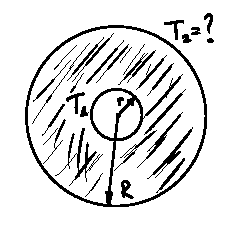
\includegraphics[width=4cm,height=4cm]{heat.pdf}
  \end{center}
  \vspace{-0.7cm}
  \caption{Тепловой поток цилиндра.}
  \label{fig:heat}
\end{wrapfigure}


В теории теплоты также очень хорошо сработает закон Гаусса. Пусть
имеется цилиндр радиусом $r$, достаточно большой длиной $L$ и
постоянной температурой $T_1$, которая поддерживается за счёт
внутренних источников (пусть это будет нагретая провоолка внутри
цилиндра). Цилиндр окружён теплопроводящим материалом с постоянной
теплопроводностью $K$. Радиус этого внешнего слоя равен $R$. Чему
равна температура на его поверхности?

Будем решать эту задачу как электростатическую, по теореме Гаусса. Из
симметрии ясно, что температура зависит только от расстояния от центра
(также как потенциал зависит только от расстояния до центра
заряженного цилиндра). Окружим наш цилиндр поверхностью радиусом $r_1$
и длиной $L$. Площадь этой поверхности равна $S = 2\pi r_1 L$. Через
эту поверхность проходит количество тепла $G = 2\pi r_1 h L$ (мы учли,
что поле цилиндрически--симметрично) --- в электростатике, как мы
помним, поток поля пропорционален электрическому заряду. В то же
время, мы можем написать, что

\begin{equation}
  \label{eq:heated_cylinder_1}
  h = -K \frac{dT}{dr_1}.
\end{equation}

Опять-таки, из-за сферической симметрии от градиента остаётся только
лишь производная по радиусу. Это уравнение легко решить: 

\begin{equation}
  \label{eq:heated_cylinder_2}
  \frac{dT}{dr_1} = -\frac{G}{2\pi K L r_1} \quad \Rightarrow \quad T_2 - T_1 =
  -\frac{G}{2\pi K L} \log \frac{R}{r}.
\end{equation}

Чему отвечает такая система в электростатике? Видно, что разность
потенциалов зависит от расстояния до центра логарифмически. Также она
зависит от параметра $G$, который в электростатике имеет смысл
электрического заряда. Таким образом, можно сказать, что наш нагретый
цилиндр --- это цилиндрический конденсатор в теории электричества.

\subsection{Гидродинамика.}
\label{sec:hydro}

Вторая задача, решение которой может быть сведено к электростатике,
--- задача о постоянном течении несжимаемой жидкости. Дело в том, что
жидкость --- очень сложная для изучения среда и необходимы очень
серьёзные приближения, чтобы можно было что-то сосчитать. Поле,
которое нас интересует в гидродинамике --- поле скорости жидкости,
$\vec{v}$. 

Во-первых, будем считать, что в изучаемой нами области у жидкости нет
источников и стоков. Если движение жидкости постоянно, то скорость
$\vec{v}$ не зависит от времени. Пусть $\rho$ --- плотность жидкости,
тогда $\rho \vec{v}$ --- масса жидкости, проходящей за единичное время
через единичную площадку. Так как процессы рождения и исчезновения
жидкости отсутствуют, то дивергенция потока массы отсутствует, т.е.

\begin{equation}
  \label{eq:hydro_1}
  \vn \cdot (\rho \vec{v}) =0.
\end{equation}

Если предположить, что жидкость однородна и несжимаема, то плотность
постоянна, и её можно вынести за знак дивергенции. Таким образом, у
нас получается уравнение, напоминающее электростатику без зарядов: 

\begin{equation}
  \label{eq:hydro_2}
  \vn \cdot \vec{v} = 0.
\end{equation}

Чтобы добиться окончательного сходства с электростатикой, нужно
потребовать, чтобы течение жидкости было безвихревым. Этого можно
добиться при определённых условиях, на которых мы сейчас не будем
останавливаться. Условие безвихревого течения выглядит так: 

\begin{equation}
  \label{eq:hydro_3}
  \vn \times \vec{v} = 0.
\end{equation}

Эти два уравнения и будут основой для установления аналогии с
электростатикой. Мы уже видим, что наш вектор $\vec{v}$ играет здесь
ту же роль, какую вектор $\vec{E}$ играет в электричестве. Можно
заключить, что существует функция $\chi$, такая что

\begin{equation}
  \label{eq:hydro_4}
  \vec{v} = - \vn \chi.
\end{equation}


\begin{wrapfigure}{r}{40mm}
  \vspace{-1cm}
  \begin{center}
    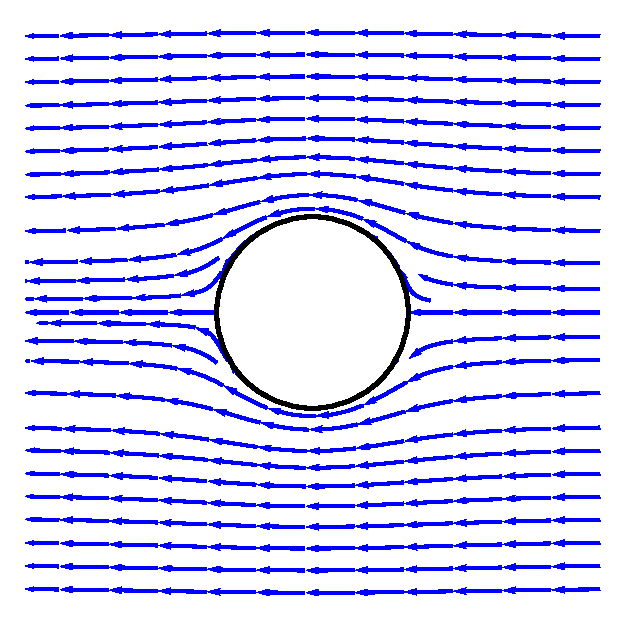
\includegraphics[width=4cm,height=4cm]{fluid_lines.pdf}
  \end{center}
  \vspace{-0.7cm}
  \caption{Обтекание шара.}
  \label{fig:hydro}
\end{wrapfigure}


Рассмотрим теперь обтекание шара нашей медленной несжимаемой невязкой
жидкостью. Примерная картика потоков жидкости приведена на
рисунке. Наша задача будет состоять в определении зависимости скорости
$\vec{v}$ жидкости от расстояния от центра шара $r$. Сначала мы найдём
<<потенциал>> $\chi$, а потом возьмём от него градиент. Каким условиям
должен удовлетворять потенциал? Во-первых, течение должно
отсутствовать за поверхностью шара, это соответствует тому, что
производная потенциала по радиусу на границе шара должна обращаться в
ноль. Во-вторых, течение на бесконечности должно переходить в
константу. Эти два условия можно записать так:

\begin{equation}
  \label{eq:hydro_bc}
  \left.\frac{\pt \chi}{\pt r} = 0\right|_{r=a}, \quad \frac{\pt
    \chi}{\pt x} = v_0, \quad r \gg a.
\end{equation}

Наша задача, таким образом, эквивалента электростатической системе без
зарядов, но с однородным электрическим полем $\vec{E}_0$, в которую
помещена диэлектрическая сфера. Если бы сферы не было, то потенциал
всюду был бы равен $\phi = - E_0 z$. Однако, у нас есть сфера, которая
всё портит. 

Мы, однако, можем воспользоваться таким фактом: если мы угадаем
решение, которое удовлетворяет уравнению Пуассона и граничным
условиям \eqref{eq:hydro_bc}, то это решение будет
единственным. Поэтому будем искать решение в виде 

\begin{equation}
  \label{eq:hydro_4}
  \phi = -E_0 x + k\frac{px}{r^3}.
\end{equation}

Здесь $p$ --- параметр, который нам ещё предстоит определить. Заметим,
что этот потенциал на больших расстояних стремится к $-E_0 x$, как и
положено, согласно второму граничному условию. Второе слагаемое в
потенциале --- потенциал диполя, и поэтому он удовлетворяет уравнению
Пуассона. Теперь надо подобрать $p$. Выразим $x$ через $r$ и угол
$\theta$, получим

\begin{equation}
  \label{eq:hydro_5}
  \phi = - E_0 r \cos \theta + k \frac{p r \cos \theta}{r^3}.
\end{equation}

Теперь приравняем производную по $r$ к нулю, получим

\begin{equation}
  \label{eq:hydro_6}
  p = -2\pi \eps_0 a^3 E_0.
\end{equation}

Заметим, что если бы два слагаемых зависели от $\theta$ по-разному, мы
бы не смогли подобрать $p$. Это доказывает правильность нашего
первоначального решения искать $\phi$ именно в таком виде. Теперь
потенциал может быть записан так: 

\begin{equation}
  \label{eq:hydro_7}
  \phi = -E_0 \cos \theta \left(r + \frac{a^3}{2r^2} \right).
\end{equation}

Чтобы получить гидродинамический потенциал $\chi$, надо просто
поменять пару букв. 

\begin{equation}
  \label{eq:hydro_8}
  \chi = - v_0 \cos \theta \left(r + \frac{a^3}{2r^2} \right).
\end{equation}

Ответ для поля $\vec{v}$ приведён на картинке \ref{fig:hydro}.

\section{Уравнения Максвелла.}
\label{sec:maxwell}

Кроме электростатических сил, в поле наших интересов находятся также
магнитные статические силы. Как мы увидим, в чём-то они очень похожи
на электростатические, а в чём-то сильно отличаются. Наша задача
сейчас --- получить законы, описывающие магнитное поле, аналогичные
теореме Гаусса \eqref{eq:statics_div_2} и теореме о роторе
\eqref{eq:rot_electrostatics_2}. 

\subsection{Сохранение энергии в электродинамике.}
\label{sec:conservation_energy}

В случае электростатики отправной точкой у нас была теорема Гаусса;
сейчас мы применим соображения из закона сохранения энергии. Для
начала нам нужно само определение \textbf{магнитного поля}. Возьмём в
качестве пробного тела маленькую магнитную стрелку, которая может
свободно вращаться вокруг своего центра масс. Измерим величину момента
вращения; эта величина пропорциональна напряжённости магнитного поля
$\vec{H}$. За направление этого поля принимается направление, в
котором устанавливается эта стрелка (считая от южного полюса к
северному). По аналогии можно определить плотность энергии магнитного
поля как

\begin{equation}
  \label{eq:def_magnetic_energy}
  U_M = \frac{\mu_0}{2} \vec{H}^2,
\end{equation}
где $\mu_0$ играет роль <<магнитной проницаемости>>, по аналогии с
$\eps_0$. 

Попробуем теперь выяснить законы, описывающие электромагнитное
поле. Рассмотрим любую часть однородного, находящегося в покое тела, в
котором образовано электромагнитное поле. Рассмотрим процесс
перетекания энергии наружу (или приток снаружи). Введём \textbf{поток
  энергии} $\vec{S}$ --- величину, которая показывает, сколько энергии
проходит в единицу времени через единичную площадку.

Примем за аксиому такой факт: вектор потока энергии (иначе называемый
\textbf{вектором Пойнтинга}) пропорционален полям $\vec{E}, \vec{H}$ и
направлен по правилу правой руки, т.е.

\begin{equation}
  \label{eq:def_pointing}
  \vec{S} = \vec{E} \times \vec{H}.
\end{equation}

% Здесь $c$ --- коэффициент пропорциональности, точный смысл которого
% выяснится позднее. 

Теперь обсудим вопрос о превращении энергии. В каждой среде
электрическая энергия непрерывно переходит в тепловую, причём
количество перешедшей в тепло энергии пропорционально плотности
электрической энергии в данном месте:

\begin{equation}
  \label{eq:def_heat_from_electric}
  dt\, dV\, \frac{\eps_0}{2} \vec{E}^2 \cdot \const \equiv dt\, dV\,
  \sigma \vec{E}^2.
\end{equation}

Константа $\sigma$, стоящая в этом выражении, зависит исключительно от
природы вещества, в котором рассеивается электрическая энергия. Она
называется \textbf{проводимостью}. Для магнитной энергии аналогичного
явления не существует.

Вычислим происходящее за элемент времени $dt$ изменение
электромагнитной энергии в какой-либо части нашего тела. Для этого
всего лишь надо взять производную от выражения, которое даёт энергию. 

\begin{equation}
  \label{eq:conserv_energy_der_1}
  dt \int dV \left( \eps_0 (E_x \dot{E}_x + E_y \dot{E}_y +
    E_z \dot{E}_z) + \mu_0 (H_x \dot{H}_x + H_y \dot{H}_y +
    H_z \dot{H}_z) \right).
\end{equation}

Это изменение обсуловлено, во-первых, притоком энергии (вместе с
вектором Пойнтинга) в количестве

\begin{equation}
  \label{eq:conserv_energy_der_2}
  dt \int \vec{S} \cdot d\vec{A} =  \int dV\, \div \vec{S} ,
\end{equation}
и во-вторых, происшедшим за тот же интервал времени образованием
тепловой энергии в количестве 

\begin{equation}
  \label{eq:conserv_energy_der_3}
  dt \int dV\, \sigma \vec{E}^2.
\end{equation}

С точностью до знака мы можем написать уравнение баланса энергии: 

\begin{eqnarray}
  \label{eq:conserv_energy_der_4}
\nn
  \frac{\eps_0}{2} \left(E_x \dot{E}_x + E_y \dot{E}_y +
    E_z \dot{E}_z \right) +   \frac{\mu_0}{2} \left(H_x \dot{H}_x + H_y \dot{H}_y +
    H_z \dot{H}_z \right) + \\
+ \div \vec{S} + \sigma \left(E_x^2 + E_y^2 +E_z^2 \right) =0.
\end{eqnarray}

Уравнение \eqref{eq:conserv_energy_der_4} представляет собой уравнение
относительно шести компонент поля и их производных. Чтобы получить из
него уравнения, описывающие поля в отдельности, можно приравнять нулю
коэффициенты при этих компонентах. Например, приравнивая коэффициент
при $E_x$ нулю, получим

\begin{equation}
  \label{eq:conserv_energy_der_5}
  \eps_0 \dot{E}_x = \left( \frac{\pt H_z}{\pt y} - \frac{\pt H_y}{\pt
      z}\right) - \sigma E_x,
\end{equation}
а при $H_x$ 
\begin{equation}
  \label{eq:conserv_energy_der_5}
  \mu_0 \dot{H}_x = -\left( \frac{\pt E_z}{\pt y} - \frac{\pt
      E_y}{\pt z}\right).
\end{equation}

Очевидно, что оставшиеся четыре коэффициента дадут похожие уравнения;
их можно объединить в векторную форму: не расписывать всё по
компонентам, а написать сразу для векторов.

\begin{eqnarray}
  \label{eq:maxwell_half}
\nn
  \eps_0 \frac{\pt \vec{E}}{\pt t} &=& \rot \vec{H} - \sigma
  \vec{E},\\
  \mu_0 \frac{\pt \vec{H}}{\pt t} &=& -\rot \vec{E}.
\end{eqnarray}

Для ещё большего упрощения этой записи можно ввести вектора $\vec{D} =
\eps_0 \vec{E}$, $\vec{B} = \mu_0 \vec{H}$, а также вектор
\textbf{тока} $\vec{J} = \sigma \vec{E}$. Возьмём теперь дивергенцию
от второго уравнения Максвелла. Дивергенция ротора в правой части
всегда равна нулю, так что получаем

\begin{equation}
  \label{eq:gauss_magnet}
  \frac{\pt}{\pt t} \div \vec{B} = 0.
\end{equation}

Это означает, что если у нас с самого начала было немагнитное тело, то
оно не сможет никогда стать источником магнитного поля (иначе
дивергенция перестала бы быть равна нулю). Одиночных магнитных
источников в природе не существует (т.е. не существует магнитных
аналогов электрических зарядов). Таким образом, полная система
уравнений, описывающая электромагнитное поле (\textbf{уравнения
  Максвелла}), выглядит так:

\begin{eqnarray}
  \label{eq:maxwell_equations}
  \nn
  \rot \vec{E} &=& - \frac{\pt \vec{B}}{\pt t}, \qquad \div \vec{B} = 0,\\
  \rot \vec{H} &=& \vec{J} + \frac{\pt \vec{D}}{\pt t}, \quad \div
  \vec{D} = \rho.
\end{eqnarray}

\subsection{Согласованность уравнений Максвелла.}
\label{sec:cons_maxwell}

Разберём несколько следствий уравнений Максвелла. Во-первых,
рассмотрим самую простую ситуацию --- статические поля. Поле
называется статическим, если его конфигурация не меняется во времени;
это означает, что производные полей по времени равны нулю. В нашем
случае это даёт уравнения

\begin{equation}
  \label{eq:statics_maxwell_1}
  \rot \vec{E} = 0, \quad \rot \vec{H} = \vec{J}.
\end{equation}

Первое уравнение означает, что электростатическое поле не имеет
циркуляции. Мы уже знаем это свойство, так что сейчас мы просто
проверили согласованность всех наших выводов. Второе уравнение следует
разобрать подробнее. 

Для того, чтобы конфигурация была статической, необходимо, чтобы ни в
одной точке пространства не осуществлялась передача тепла. Таким
образом, есть ещё дополнительное условие: $\sigma \vec{E}^2 =
0$. Таким образом, либо проводимость $\sigma$ должна равняться нулю,
либо само поле $\vec{E}$. В любом случае, ток тоже будет равен нулю,
так что получаем

\begin{equation}
  \label{eq:statics_maxwell_2}
  \rot \vec{H} = 0.
\end{equation}

Таким образом, магнетостатика и электростатика распадаются на два
совершенно независимых семейства уравнений, что позволяет говорить о
наложении электрических и магнитных полей. 

\section{Магнетостатика.}
\label{sec:magnetostatics}

Посмотрим теперь, как будут выглядеть магнитные поля в стационарном
случае (т.е. когда производные полей по времени равны нулю, но ток
может протекать). Для начала введём \textbf{магнитный потенциал}
$\vec{A}$. Заметим, что так как $\rot \vec{B} = 0$, то существует
такой вектор, что 

\begin{equation}
  \label{eq:def_vector_potential}
  \vec{B} = \rot \vec{A}.
\end{equation}

Подставляя это соотношение в уравнения Максвелла
\eqref{eq:maxwell_equations}, получаем 

\begin{equation}
  \label{eq:laplace_vector_pot_1}
  \rot \rot \vec{A} = \mu \vec{J}.
\end{equation}

Заметим теперь, что вектор $\vec{A}$ определён неоднозначно: мы можем
добавить к нему градиент любого скаляра, и ничего не изменится (это
называется \textbf{калибровочной инвариантностью}). Чтобы всё-таки
как-то зафиксировать вектор $\vec{A}$, можно наложить на него,
например, такое условие: $\div \vec{A} = 0$. 

Далее, можно преобразовать уравнение
\eqref{eq:laplace_vector_pot_1}. Заметим для этого, что $\rot \rot
\vec{A} = \grad \div \vec{A} - \Delta \vec{A}$. Таким образом,
получаем для нашего вектор--потенциала: 

\begin{equation}
  \label{eq:laplace_vector_pot_2}
  \Delta \vec{A} = - \mu \vec{J}. 
\end{equation}

Заметим, что это уравнение очень похоже на уравнение Пуассона для
скалярного потенциала \eqref{eq:poisson_3}. А раз мы знаем решение
уравнение Пуассона для $\phi$, то можем легко по аналогии написать
решение уравнения для $\vec{A}$: 

\begin{equation}
  \label{eq:solution_vector_pot}
  \vec{A}(\vec{r}) = \int \frac{\vec{J}(\vec{r'})}{r} d\vec{r'}.
\end{equation}

Это выражение --- точная аналогия выражения для потенциала от
произвольной системы зарядов. 
\end{document}